
\section{Learning from Demonstrations}
\label{sec:lfd}

\subsection{Introduction}


 Several studies have examined how people walk and climb stairs. Motion capture is one tool used for recording human kinematics and kinetics. In  \cite{chalodhorn2007learning}, Chalodhorn \textit{et. al} used a model-free approach to teach a robot to walk. In  \cite{hu2014online}, Hu \textit{et. al} used quadratic programming to optimize the mapping of the markers to the robot. Motion capture mapping was used to map from a human to a humanoid robot in both cases. This research was limited to direct robot control, and the robot was only able to perform the exact motion of the human.

 In \cite{taskjointmocap}, Hu \textit{et. al} focused on online generations of trajectories. They formulated the control problem as a Quadratic Programming (QP) problem, and the authors used both Cartesian and joint data as the imitation criteria. The formulation as a QP problem allows for inequality and equality constraints for the knee velocity. This formulation resolves the conflicts between the joint space and the Cartesian imitation data. This method is limited to level ground walking. This process did not address abstracting the trajectories for different stair heights; it only addressed level ground walking and fully actuated systems.
 
 Learning from Demonstration allows for complex motions to be learned and reproduced on robotics systems; this enables the desired motion to be taught to the exoskeletons instead of hand-generating the gait motion needed to accomplish the same goal. This section will show how to use human gait demonstrations to learn and reproduce a gait motion and generate a trajectory to climb stairs.  


\subsection{Overview of methods and applications}
Learning from Demonstration (LfD) is the process of transferring skills to a robot by demonstration. In \cite{siciliano2016springer}  \cite{kormushev2011imitation} \cite{calinon2007teacher} Calinon \textit{et al} outline the process of teaching a robot how to follow a trajectory. There are several steps of LfD: demonstration modality, motion primitives, and encoding methods. There are several steps of the LfD process, as stated below. 

\begin{enumerate}[noitemsep]
    \item Recognition of the task 
    \item Encoding of the motion 
    \item Retrieval of the task 
    \item Reproduction of task 
\end{enumerate} 

There are primary teaching modalities that can be sorted into two teaching methods. These modalities are used to teach a robot to follow a trajectory and collect data. The first teaching modality is kinesthetic teaching. This modality involves a user moving a robot passively or running an impedance controller through a task while recording the joint positions and torques \cite{Calinon2018}. Researchers have applied kinetic teaching for upper limb robotic systems for industry and human-robot interfaces. While this method is a natural teaching method, it is not well suited for teaching lower limb movement because it would require directly moving a leg through a gait motion. It would be difficult to replicate the leg's motion by the manual moving of a person or robot. 

The second teaching modality is visual observation. In this teaching modality, visual sensors record the desired motions and intentions of a demonstration for mapping onto a robotic system \cite{CalinonLee19}. In visual observation, mocap is the standard method. The marker system allows for precise tracking of points on a person with millimeter accuracy \cite{ott2008motion}. This method has broad adaptation capabilities and high accuracy for gait data collection \cite{ViconGaiting}.

Dynamic Motion Primitive (DMP) is a method of breaking down demonstrations into their fundamental building blocks; it is a popular form of motion primitive \cite{ijspeert2013dynamical}. Motion primitives aim to encode trajectories into building blocks that can be rearranged and manipulated. DMP works by creating a stable underlying model and generating a forcing function to drive the system.  

There are several LfD methods for learning trajectories and building models based on the data from the two teaching modalities, including Locally Weighted Regression (LWR), Hidden Markov Models (HMM), and Gaussian Mixed Regression (GMR). They are all methods of encoding motion into basis functions for learning and reproduction. These methods are similar, but each method contains its unique pros and cons. LWR is the simplest method, with HMM and GMR being extensions of this method. HMM and GMR places the radial basis functions (RBF) on the trajectory more effectively.  

HMM combines temporal scaling and transition probabilities through a double stochastic process \cite{calinon2007learning}. HMM has built-in temporal scaling, meaning that it can deal with demonstrations that are not aligned. The double stochastic process makes it challenging to retrieve smooth and continuous trajectories; this makes it unsuitable for teaching exoskeleton trajectories, as stated by Calinon \textit{et. al}. The GMM method produces smooth and continuous trajectories, making it better suited for producing trajectories for exoskeletons. 

The GMR method uses GMM to provide a more comprehensive approach to the RBF placement and allows for the encoding of multiple trajectories \cite{calinon2013compliant}. GMM is similar to K-means; however, it uses the Expectation-Maximization (EM) algorithm to find the optimal placement of the RBF on the data set. GMR is used to regress the RBFs to find an underlining model. The demonstrations require temporal alignment before being encoded. Dynamic Time Warping temporally aligns two demonstrations (DTW). The DTW algorithm attempts to minimize the distance between two trajectories by drawing lines between the two curves \cite{muller2007dynamic} \cite{JSSv031i07}. 
 GMR is computationally fast and produces smooth and continuous trajectories. The benefits of using GMR are the following \cite{Calinon}: 


\begin{enumerate}[noitemsep]
    \item Allows encoding of local correlation between motion variables
    \item Provides a principled approach to estimate the parameters of the RBF 
    \item Reduce the number of RBF   
    \item Online estimation of the DMP parameters and model selection   
\end{enumerate}  

There are four steps for building the imitation model listed below. \autoref{fig:demostation} illustrates the workflow for training and reproduction.

\begin{enumerate}[noitemsep]
    \item Collection of gait data
    \item Encoding of motion into RBF
    \item Learning of regression function
    \item Reproduction, and manipulation of the trajectories
\end{enumerate}


\begin{figure} 
    \centering 
    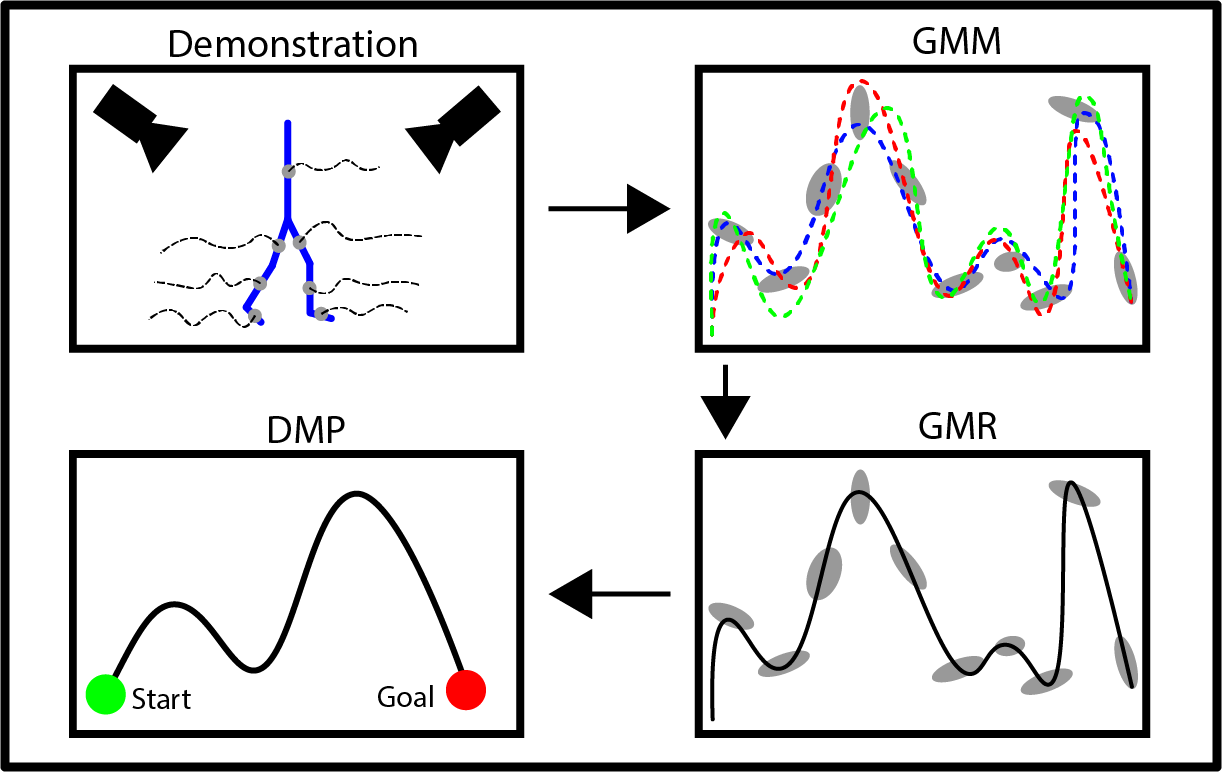
\includegraphics[scale=0.25]{images/background/demo_figure.png} 
    \caption[Learning Process]{Order of operations of the learning process. The data is collected, the demos are encoded and aligned with DTW, the model is retrieved, then the model is reproduced.} 
    \label{fig:demostation} 
\end{figure} 


In the classical formulation of DMPs, the model places radial basis functions (RBF) along the single demonstration to pull the system towards the goal. GMR/GMM replaces this method with a methodical placement of the RBFs and multiple demonstrations to train the model. DMPs are considered one of the gold standards of learning and replicating human motion \cite{nakanishi2004learning}.


To compare and encode the demonstrations, they must be the same length. When recording live motion data, the demonstrations of the same task will be of different lengths depending on how fast the subject moves; this will create demonstrations that are similar in motion but are not temporally aligned. These demonstrations could be aligned by re-sampling the trajectories to be the same length. However, there is no guarantee that the features of the trajectories will align after they are re-sampled. This problem can be resolved by using Dynamic Time Wrapping, which provides a principled approach to align demonstrations by finding the minimum distance between each point of the demonstrations \cite{JSSv031i07}. DTW ensured that similar parts of the trajectories aligned with each other. 

\subsection{Mathematics of Learning}
 

 \autoref{eq:DTW} shows the equation for DTW; it maps demo 2 onto demo 1. Here, $\delta (P, T)$ is defined as the Manhattan distance function. $P$ and $T$ are demo 1 and demo 2, respectively. This method maps $P$ onto $T$ . Here, $w_k$ is the cost at index $(i,j)$, and $k$ is the time frame.
 
 \begin{equation} 
    \begin{aligned} 
         \delta (P,T) &= | p_i - t_j| & \text{Distance function} \\ 
        DTW(P,T) &= min \Bigg[ \sum_{k=1}^{K} \delta (w_k) \Bigg] & \text{Minimum path} 
    \end{aligned} 
    \label{eq:DTW} 
\end{equation} 

 
 
 \autoref{fig:DTW_example} illustrates how DTW functions. Here two $cosine$ functions of different lengths are aligned. The cost matrix path shows that the demonstrations are aligned. Each of the axis in the cost matrix diagram are the two demonstrations. The path is the minimum cost through the matrix. The illustration shows one of the primary problems with DTW; the time-wrapped trajectory (green line) has sharp bends in the line, it does not produce smooth trajectories. This problem can be solved by fitting a polynomial to the time-wrapped trajectory shown as the red line.  
 
 \begin{figure}[htb!]
     \centering
     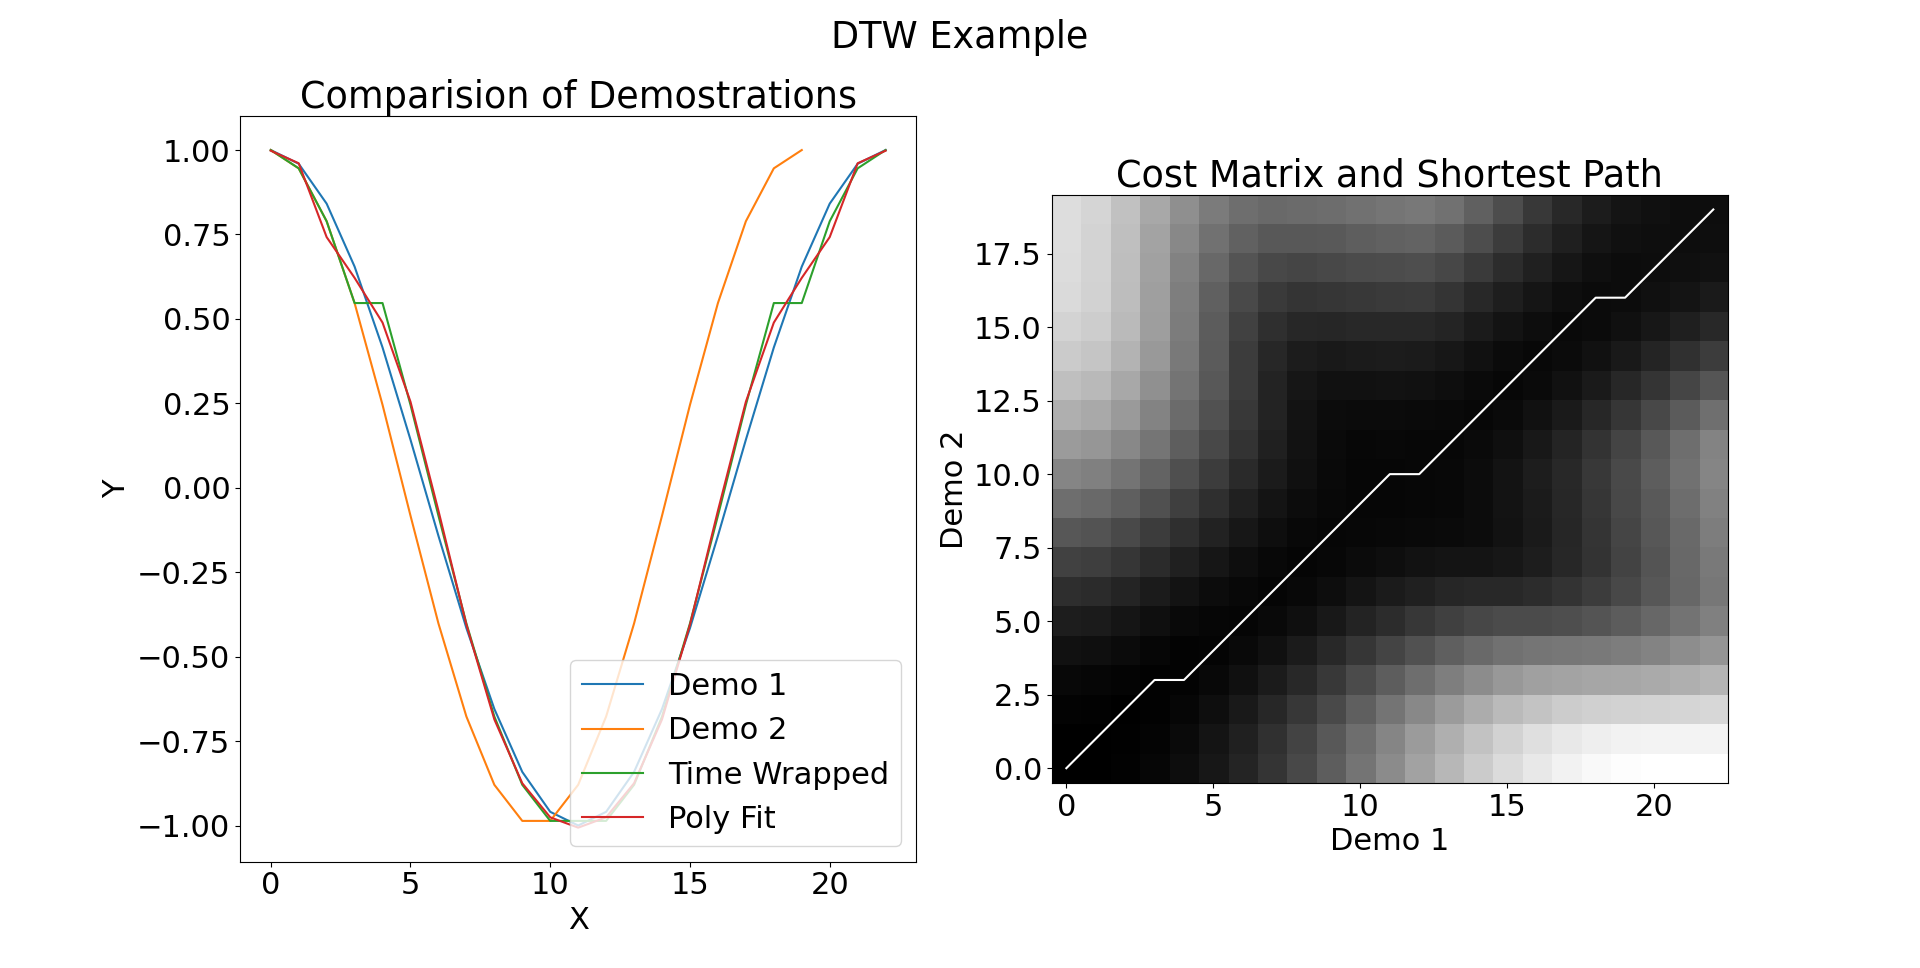
\includegraphics[scale=0.3]{images/background/DTW_example.png}
     \caption[DTW Example]{Two demos being aligned using DTW and a smoothed trajectory. Blue line: demo 1. Orange line: demo 2. Green line: aligned trajectory. Red line: Poly Fit The cost map shows the distance between the points. }
     \label{fig:DTW_example}
 \end{figure}



DMPs work by developing an underline stable motion model and adding a forcing function to drive the system along the trajectory. \autoref{eq:DMP_Model} control how the system moves along the trajectory, where $\alpha_y$ and $\beta_y$ are gains and $y$ is the system state. This system acts as a PD controller. The forcing function $f$ drives the systems by placing RBF along the trajectory and attracting the system to the points. The forcing functions is built using \autoref{eq:DMP_force}. Here $w_i$ is the weighting on the basis function $\psi_i$ defined by the Gaussian's centered at $c_i$ where the $h_i$ is the variance. As the system moves along the trajectory, the Gaussians are activated and pull the system. DMPs are limited to the use of a single demonstration for training.  

\begin{equation}
    \Ddot{y} = \alpha_y ( \beta_y ( g - y) -\Dot{y}) + f
    \caption{DMP model}
    \label{eq:DMP_Model}
\end{equation}


\begin{equation}
 \begin{split}
    \Dot{x} &= -\alpha_x x \\
    f(x,g) &= \frac{\sum_i^N \psi_i w_i}{\sum_i^N \psi_i}x(g-y_0)\\
    \psi &= \exp( -h_i (x -c_i)^2)
 \end{split}
    \caption{DMP model}
    \label{eq:DMP_force}
\end{equation}

The GMM method uses the EM algorithm that iteratively updates the probabilities of the points.  \autoref{eq:Estep} and \autoref{eq:Mstep} show the two steps in the EM algorithm. In these equations, $X$ is the point vector, $h$ is the posture probability, $\pi$ is the weighting coefficient for each point, $\mu$ is the mean, and $ \Sigma $ is the covariance. K-means is used to find the initial guess of the $\mu$ and $\Sigma$ parameters for the EM algorithm with the value of $\pi$  initialized randomly. 

E(xpectation)-step:


\begin{equation} 
    \centering
     h_{t,i} = \frac{\pi_i \prod_{j=1}^{P} \mathcal{N}(X_t^j | \mu_i^j , \Sigma_i^j )}{ \sum_k^K \pi_k \prod_{j=1}^{P} \mathcal{N}(X_t^j | \mu_k^j , \Sigma_k^j ) } 
     \label{eq:Estep} 
\end{equation}{} 

M(aximization)-step: 
\begin{equation} 
\begin{aligned} 
    \pi_i &\leftarrow \frac{\sum_t^N h_{t,i}}{N} \\ 
    \mu_i^j &\leftarrow \frac{\sum_t^N h_{t,i} X_t^j}{\sum_t^N h_{t,i}} \\ 
    \Sigma_i^j &\leftarrow \frac{\sum_t^N h_{t,i} ( X_t^j - \mu_i^j)  ( X_t^j - \mu_i^j)^T   }{\sum_t^N h_{t,i}}  
\end{aligned} 
\label{eq:Mstep} 
\end{equation} 



TPGMM is similar to the Gaussian mixed model (GMM); the difference between TPGMM and GMM is that TPGMM models the importance of a task in the frame rather than the constant Gaussian ($\mu_$, $\Sigma_i$). The model is defined by $ \{ \pi_i \{ \mu_i^j , \Sigma^j \} _{j=1}^P \}$, $\pi_i$ is the mixing coefficient, $\mu$, is the mean, and $\Sigma$ is the covariance matrix of the Gaussian.
 The EM equations are altered to handle the importance of a task in the frame. The altered  E-step and M-step are shown in \autoref{eq:EstepTPGMM} and \autoref{eq:MstepTPGMM}.

E(xpected)-Step:
\begin{equation}
    \gamma_{n,i} = \frac{\pi_i \prod_{j=1}^{P} \mathcal{N}( X_n^j | \mu_i^j, \Sigma_i^j)  }{   \sum_{k=1}^{K} \pi_k \prod_{j=1}^{P} \mathcal{N}( X_n^j | \mu_i^j, \Sigma_i^j)}
    \label{eq:EstepTPGMM}
\end{equation}

 M(aximization)-Step:
 
\begin{equation} 
\begin{aligned} 
    \pi_i &= \frac{\sum_t^N \gamma_{t,i}}{N} \\ 
    \mu_i^j &= \frac{\sum_t^N \gamma_{t,i} X_t^j}{\sum_t^N \gamma_{t,i}} \\ 
    \Sigma_i^j &= \frac{\sum_t^N \gamma_{t,i} ( X_t^j - \mu_i^j)  ( X_t^j - \mu_i^j)^T   }{\sum_t^N \gamma_{t,i}}  
\end{aligned} 
\label{eq:MstepTPGMM} 
\end{equation} 


The covariance matrix is square and of size $N+1$, where $N$ is the number of trajectories to be trained, where the first element is the time relationship. Illustrated in \autoref{fig:cov_mat}, the covariance matrix used to calculate the Gaussian are $2x2$ sub-matrix of the larger matrix. They are constructed using the time element with the current training model $T$ for all training trajectories $1..N$. The number of matrix $K$ is detriment by the number of bins set. The sub-covariance matrix determines the shape and size of the gaussian ($\Sigma$), where the mean  ($\mu$) determines the location along the trajectory. 


\begin{figure}
    \centering
    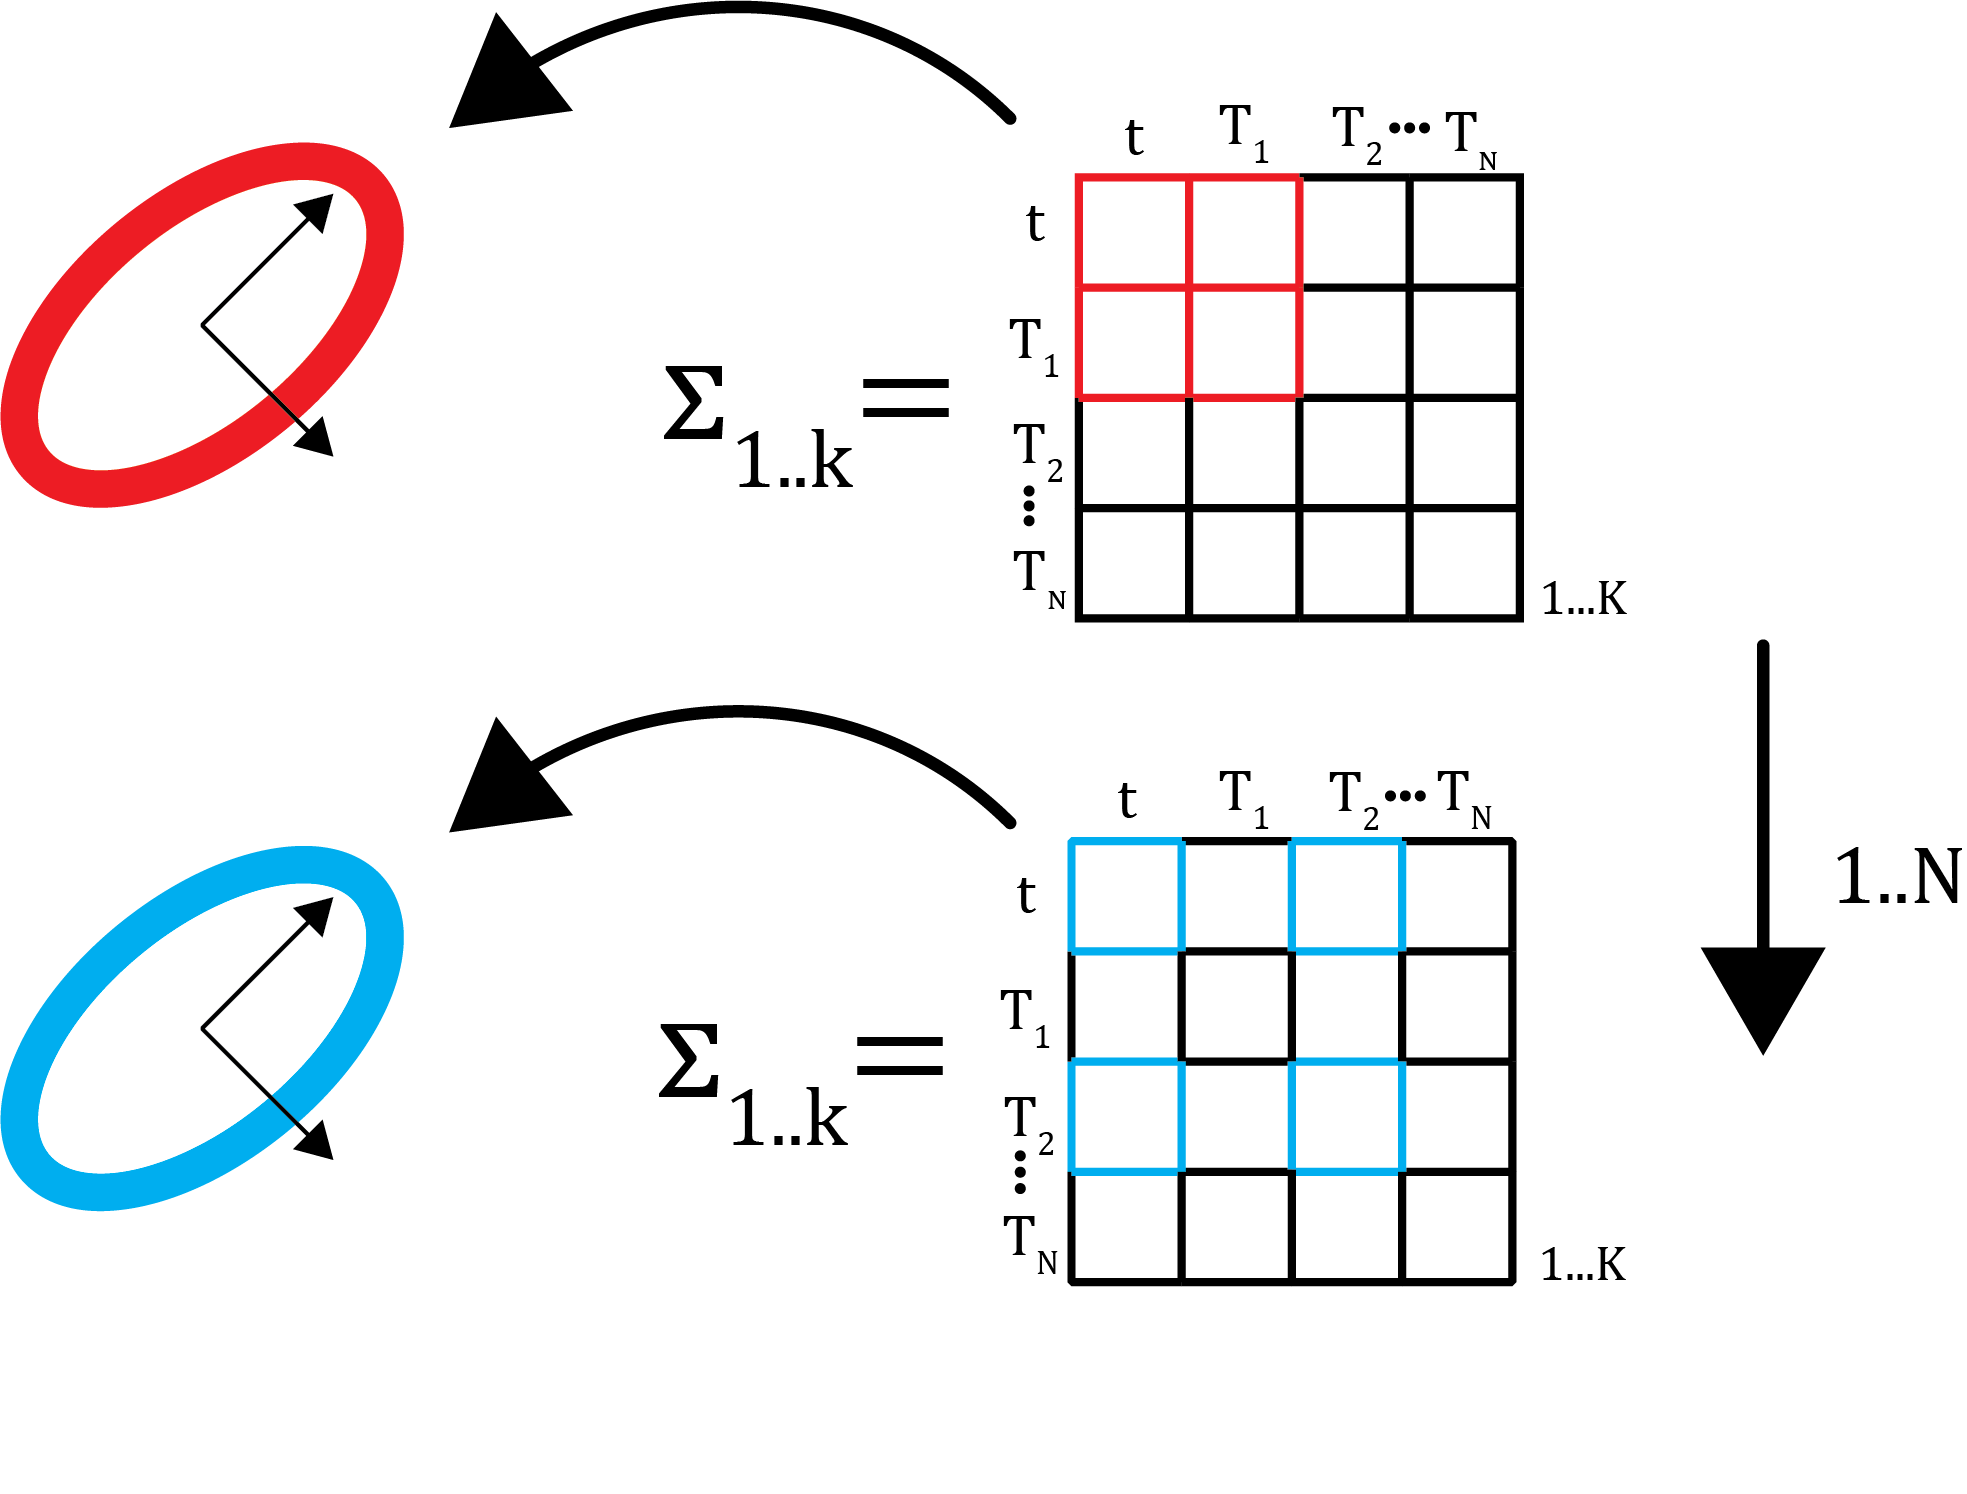
\includegraphics{images/background/cov_matrix.png}
    \caption[Covariance Matrix Illustration]{Using the covariance matrix ($\Sigma$) to calculate the gaussian for each of the trajectories}
    \label{fig:cov_mat}
\end{figure}



Each of the demonstrations $d \in \{1...D \}$ is a vector of time-sequenced data points and is of $T_d$ size. This results in a data structure of size $\sum_{d=1}^D T_d$. The length of each of the $T_i$ vectors will be different for each demonstration; this results from the subjects' stride speeds. The task parameters are represented as a coordinate system $P$ defined at each time step n defined by $\{ b_{n,j}, A_{n_j} \}^{P}_{j=1}$. The $b$ vector is a set of basis vectors from the origin with the transformation matrix $A$. This formulation allows for trajectories to be transformed into any frame using \autoref{eq:transform}. $\xi$ is the vector of the data points.

\begin{equation}
    X_t^j = A^{-1}_{t,j} ( \xi_t - b_{t,j})
    \label{eq:transform}
\end{equation}



 \autoref{eq:GMR_Prop} calculates the likelihood, and \autoref{eq:GMR_mu} calculates the covariance and mean. Where $\xi_$ is a multidimensional array, $\mu_i^o$, and $\Sigma_t^o$ are vectors of the output mean, and covariance, $\mu_i^I$, and $\Sigma_t^I$ are vectors of the input mean and covariance. 
GMR models the regression function from the joint probabilities in the form of GMM. 

\begin{equation} 
     P(\xi_t^O | \xi_t^I ) \sim \sum_i^K h_i(\xi_t^I) \mathcal{N}( \hat{\mu_i^o}, \hat{\Sigma_t^o}) 
     \label{eq:GMR_Prop} 
\end{equation} 

where, 

\begin{equation} 
    \begin{aligned} 
      \hat{\mu_i^o} &= \mu_i^o + \Sigma_i^{OI}\Sigma_i^{I-1}(\xi_t^I - \mu_i^I)\\ 
      \hat{\Sigma_i^O} &= \Sigma_i^O - \Sigma_i^{OI}\Sigma_i^{I-1} \Sigma^{IO}_i \\ 
       h_{i} &= \frac{\pi_i \mathcal{N}(\xi_t^I | \mu_i^j , \Sigma_i^j )}{ \sum_k^K \pi_k \mathcal{N}(\xi_t^I | \mu_k^j , \Sigma_k^j ) }   
    \end{aligned} 
    \label{eq:GMR_mu} 
\end{equation} 

The number of bins $ K $ used in TPGMM are found using the Bayesian Information Criterion (BIC); if too few bins are used, the model will be poorly fit; if too many are used, it will over-fit the demonstrations. BIC is a method to overcome this limitation and find the optimal number of bins \cite{calinon2007learning}. \autoref{eq:BIC} calculates the BIC score; it is a trade-off between optimizing the likelihood and minimizing the number of states to encode. $\mathcal{L}$ is the log-likelihood, $ N $ is the number of mixture models, $ K $ is the number of components, and $ D $ is the dimension of the data points. 


\begin{equation} 
    S_{BIC} = -\mathcal{L} + \frac{log(N)(K(D+1)(D+2)-2)}{4}  
    \label{eq:BIC} 
\end{equation} 


A reproduction model's accuracy is measured by calculating the imitation cost; this is essentially a root mean squared algorithm that measures how well the model follows the demonstrations \cite{metric}. \autoref{eq:metric} shows the equation used to calculate the goodness of fit. In this equation, $d$ is the demo, $m$ is each of the demos, $t$ is the time, and $x$ is the trained model. 

\begin{equation}
    C = \frac{1}{MT} \sum_m^M{\sum_t^T{ || d^m_t - x_t||}}
    \label{eq:metric}
\end{equation}


 \begin{figure}
     \centering
     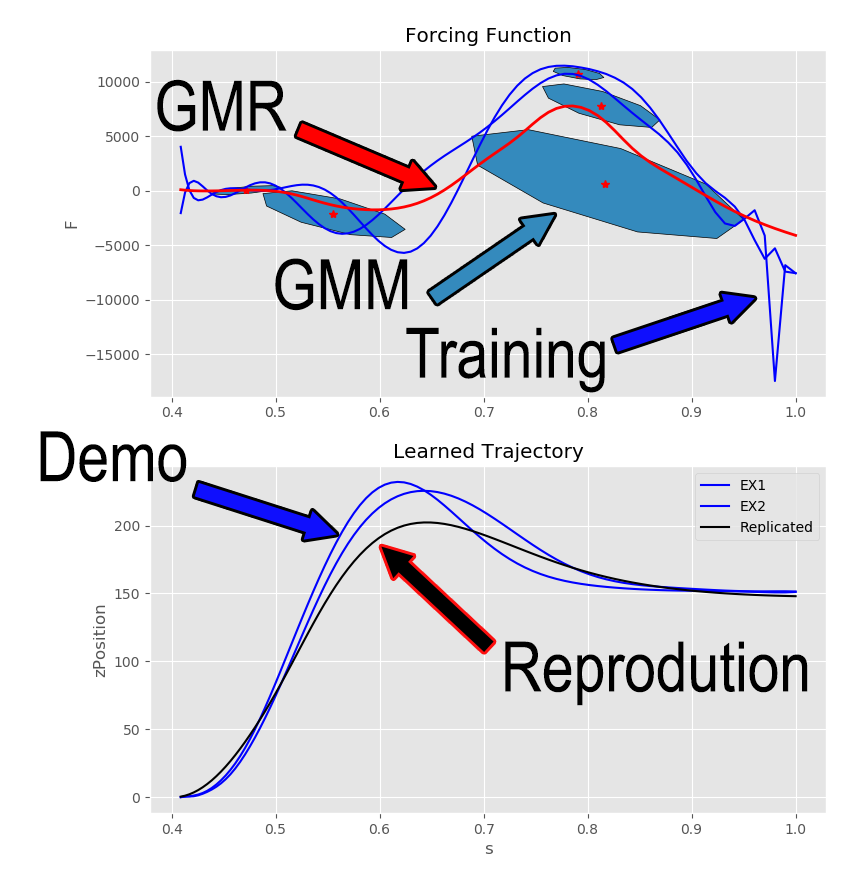
\includegraphics[scale=0.42]{images/background/GMM_reproduction.png}
     \caption[Simple Reproduction Example]{Demonstration of how LfD reproduces trajectories with the labeled components. This Model was generated using two demonstrations collected from stair climbing data. }
     \label{fig:SimpleGMMExample}
 \end{figure}

\subsection{Applications of LfD}
\label{sec:applfd}
Learning from Demonstration has been used to teach robots a variety of complicated tasks and motions. In \cite{mulling2013learning}, they used motion primitives to train a robot to play table tennis. Similarly, it was used to teach a robot to reach and grasp various objects such as balls and chess pieces \cite{calinon2007active}  \cite{hersch2008dynamical}. It has also been used to learn handwriting \cite{kulvicius2011joining}. All of these tasks share a biological movement as their training set. The robots need to replicate a complex human-like motion that would otherwise be difficult to hand code. The learning from demonstration framework allows for a human demonstration to be collected and encoded onto the robotic system to teach the required movement.  

Learning from Demonstration has not yet been explored to the fullest for imitating lower body motion. Using human demonstration and motion capture offers several advantages over other methods. The high accuracy and rich data set offer the ability to study both the inverse and forward kinematics of the person's legs and trunk, which allows for learning the joint angles or foot position; this is used to train the exoskeleton for different activities of daily living including walking and stair climbing. The difficulty arises in mapping the joint motion and how to learn the motion. Using the joint angle ignores the foot placement, while using the foot's location disregards the joint angles. Both of which are important when maintaining balance and natural joint motion. In addition, a person's joints cannot move through the desired motion as an arm, so external motion must be mapped onto the person who will have different leg lengths. 



% Stair climbing is a non-linear motion. Ascending stairs require one foot to remain on the ground while the other foot swings through a trajectory\cite{hicks2012temporal}. Several studies have examined how people climb upstairs. Motion capture is one tool that can be used for recording human kinematics and kinetics. In  \cite{chalodhorn2007learning}, Chalodhorn \textit{et. al} used a model-free approach to teach a robot to walk. In  \cite{hu2014online}, Hu \textit{et. al} used quadratic programming to optimize the mapping of the markers to the robot. In both cases, the motion capture mapping was mapped from a human to a humanoid robot. This research was limited to direct robot control, and the robot was only able to perform the exact motion of the human.

%  In \cite{taskjointmocap}, Hu \textit{et. al} focused on online generations of trajectories. They formulated the control problem as a Quadratic Programming (QP) problem, and the authors used both Cartesian and joint data as the imitation criteria. The formulation as a QP problem allows for inequality and equality constraints for the knee velocity. This formulation resolves the conflicts between the joint space and the Cartesian imitation data. This method is limited to level ground walking. This process did not address abstracting the trajectories for different stair heights; it only addresses level ground walking and fully actuated systems.
 
%  Using the foot's position to train an exoskeleton to replicate the stair climbing motion allows for the reproduction of natural biological movement and the abstraction of the stair height. The existing methods are improved using human motion to define the trajectories instead of random motion generation and can be used to move the foot to different stair heights. 
 
%  This method, however, offers several challenges. The first challenge is how to find the joint angles from the foot position for various people. While the Cartesian position of the foot is controlled, the only actuation is in the joints. The joint angles need to be found for people of various heights; this complicates the process because it adds a layer of abstraction. Another challenge is dealing with the collision with the environment. While controlling the foot, it should not collide with an object; this problem must be tackled for robotic manipulators but not for controlling lower limb robotic systems. Using learning from demonstration to control lower limb robotic platforms has the complexity necessary for varying joint lengths and collisions with the environment. Both of these problems remain unexplored and need further research.  
